\chapter{Convolutional neural networks}
\label{cnn}

\setcounter{secnumdepth}{1}

Although it is assumed that the reader has sufficient prior knowledge of artificial neural networks and convolutional neural networks, this part briefly introduces convolutional neural networks, their layer types and few selected architectures. 

For better understanding of the topic, it is recommended to take a look at the holy book of deep learning, \cite{dl}.

\section{Introducing convolutional neural networks}
\label{understanding-cnn}

If you try to find an introduction to \zk{CNN}s on the internet, you may bump into a common statement that \zk{CNN}s are neuroscience-based deep neural networks using convolution and presumpting the input is an image. It is not exact. 

Though images are the most common input, according to \cite{dl}, \zk{CNN}s presumpt the input has a grid-like topology; apart from the computer vision, other applications include  for example natural language processing (as in \cite{cnn-nlp}) or anything representable as a grid-like topology (audio waveform as 1-D grid, RGB images as multichannel 2-D, CT scan as 3-D, etc.). 

A paradox inexactness is the term \textit{convolution} as in mathematical meaning, many \zk{CNN}s implement cross-correlation instead of real convolution. Cross-correlation may be seen as convolution without a kernel flipping. The reader can get more mathematical insight about the difference and harmlessness of this change from \cite{dl}. 

It is true that \zk{CNN}s are based on a neuroscience. They are inspired by Nobel prize laureates Hubel's and Wiesel's research on mammalian vision systems (firstly cats in \cite{hubel-cats1} and \cite{hubel-cats2}, later monkeys in \cite{hubel-monkeys}). Hubel and Wiesel found that some neurons (sorted in columns) strongly respond to specific to specific edge-like patterns but just a bit to other patterns. 

The eye stimulus on the retina is transferred through the optic nerve and the lateral geniculate nucleus into the primary visual cortex (sometimes referred to as V1), a part of the visual cortex located in the posterior pole of the occipital lobe. The primary visual cortex is organized in a 2-D spatial map representing visual stimuli from the retina and contains two cell types, simple cells and complex cells. Simple cells purpose is to compute a linear function (although some counterarguments against the linearity have been raised, see \cite{simple-cells}) of the image in a spatially localized field, while complex cells operations are to some extent position and lighting invariant. 

\section{Layer types}
\label{layers}

While the common approach in image processing of classical \zk{ANN}s is to vectorize the input, \zk{CNN}s emulate the neuroscientific approach outlined in chapter \ref{understanding-cnn} using feature maps (each color channel is a feature map). \zk{CNN}s profit from the fact that pixels in an image are ordered according to some structure. That allows neurons in layers to be connected just to certain region instead of heavily arduous fully-connected architecture. 

\zk{CNN}s consist from many layers with different functions. In the following, individual layer types are briefly described. 

\subsection{Convolutional layers}
\label{conv-layers}

The first layers through which is the input passed are convolutional layers. So, firstly, what is the convolution? 

In the geomatics field, we very often encounter the term \textit{kernel}. Kernel can be seen as a matrix (or a window) sliding across all the image pixels. The pixels contained in this window are a receptive field. As both the kernel and the receptive field are matrices of the same shape, in each position element wise multiplication is computed and outputed as an output matrix element. Because after such a filtering, the output matrix contains a 2-D activation map (a map where each position values say with witch probability the requested feature is on that position in the original image), the output is called a feature map. Kernels / filters are the subject of training. 

In case of stride 1 and without zero-padding, the feature map is naturally of shape $[original\_width - kernel\_width + 1] \times [original\_height - kernel\_height + 1]$. An example may be seen in figure \ref{fig:conv}. 

\begin{figure}[H]
   \centering
	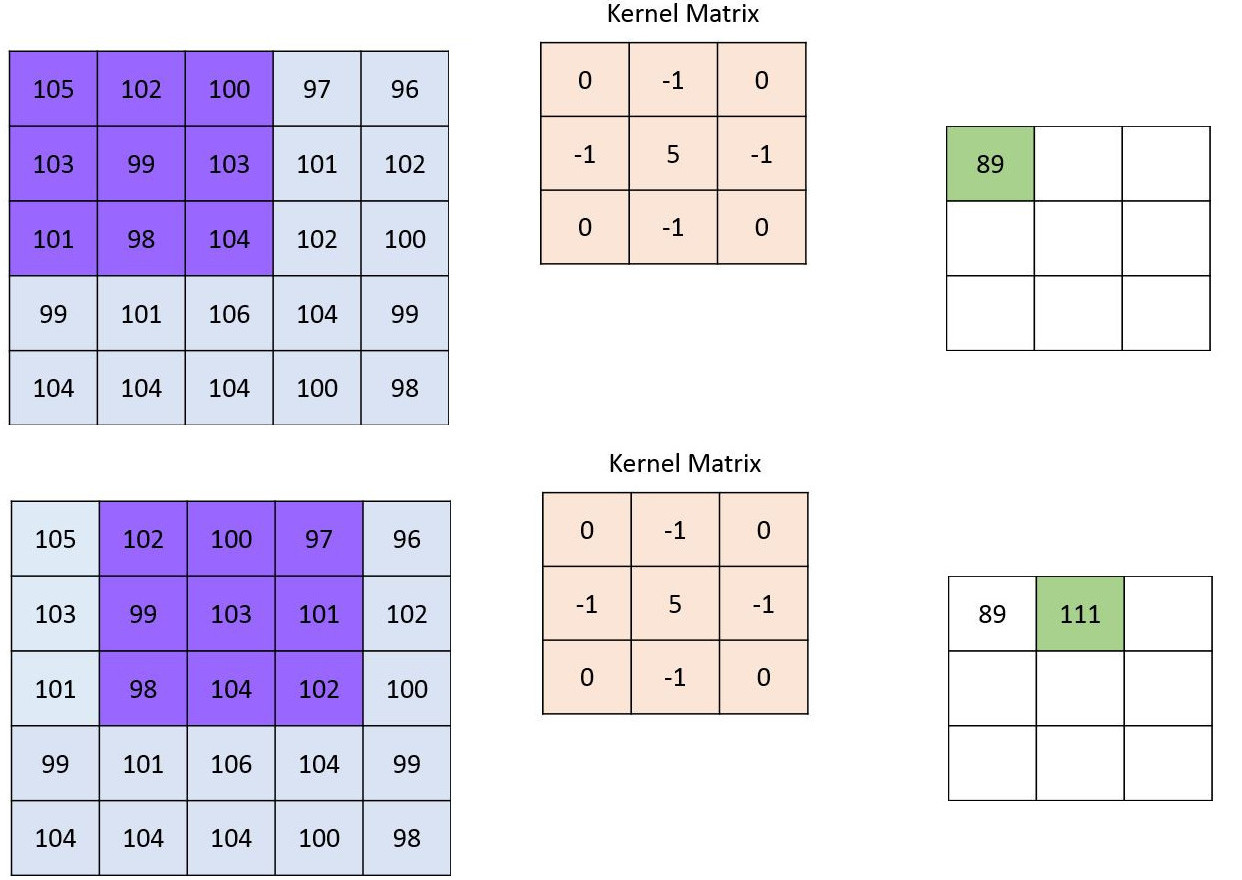
\includegraphics[width=.4\linewidth]{./pictures/conv.jpg}
	\caption[Two steps of kernel convolution]{Two steps of kernel convolution}
      \label{fig:conv}
\end{figure}

With convolution, we reduce both computational requirements and a threat of overfitting by using local connections (representing weights) between input and output. However, these connections are local only in two dimensions, in width and height of the input; these connections have to be full along the channels depth - e.g. in RGB images, the last dimension of connections is always 3. Different is it with the output; its third dimension is determined by the number of neurons referencing the same spatial location, e.g. by the number of kernels we use. 

In chapter \ref{understanding-cnn}, translational invariance was mentioned. In convolutional layers, this invariance was achieved by another huge parameter reduction, by parameter sharing. Idea of parameter sharing raised from the premise that when one feature is useful in one location, it could be useful also in another one. This simple presumption which works except for for example centered special structures allows sharing a set of parameters throughout the whole depth slice. 

Using the parameters from \cite{conv-imagenet} as an example, assumpt that the feature map has size $55 \times 55 \times 96$ and we apply it on images of size $227 \times 227 \times 3$ using kernels of size $11 \times 11 \times 3$. Sharing parameters within a depth slice, we can reduce the parameter amount from $55 * 55 * 96 * (11 * 11 * 3 + 1)$ to $96 * (11 * 11 * 3 + 96)$ (1 and 96 are biases), it means from more than 105 millions to less than 35 thousands. Speaking only about the first layer. I believe that this example said it all. 

An inquiring reader may raise a question: In the chapter name, there is a plural. What happens in deeper layers? 

Their input is the previous layer output. Output of the first layer is the feature map of the lowest level features. As was already mentioned, each neuron of the next layer is connected with some local neighbourhood and with everything along the third dimension; and because the third dimension of the output is formed by stack of filters / kernels of the first layer, each second layer neuron is connected to all detected features in some location and its neighbourhood. The result? Output feature map from the second layer contains higher level features (simple combinations of the low level ones, like triangles or squares, simply combinations of some edges, curves, etc.). The next layer will output again higher level features and in the end, we may have very specific features like cars, reflective heliports or art deco swimming pools. 

\subsection{ReLU layers}
\label{relu-layers}



\subsection{Subsampling layers}
\label{subsampling}

\subsection{Normalization layers}
\label{norm-layers}

\subsection{Fully connected layers}
\label{fc-layers}

\section{Architectures of convolutional neural networks}
\label{cnn-architectures}

\subsection{LeNet5} %
\label{lenet}

\subsection{Dan Ciresan Net}
\label{ciresan}

\subsection{AlexNet} %
\label{alexnet}

% CS231n about zero-padding

\subsection{ZF Net}
\label{zfnet}

\subsection{VGG} %
\label{vgg}

\subsection{Network-in-network}
\label{nin}

\subsection{GoogLeNet}
\label{googlenet}

\subsection{Inception V3}
\label{inception}

\subsection{ResNet} %
\label{resnet}

\subsection{SqueezeNet}
\label{squeezenet}

\subsection{ENet}
\label{enet}